\documentclass[12pt,letterpaper]{article}
% The usepackage tell LaTeX which packages are needed. As you get better you can add more
% packages for extra functionality
% Percent signs are comments, they will not be read by the renderer.
\usepackage{fullpage}
\usepackage[top=2cm, bottom=2.5cm, left=2.5cm, right=2.5cm]{geometry}
\usepackage{amsmath,amsthm,amsfonts,amssymb,amscd}
\usepackage{lastpage}
\usepackage{enumerate}
\usepackage{fancyhdr}
\usepackage{mathrsfs}
\usepackage{xcolor}
\usepackage{graphicx}
\usepackage{multicol}
\usepackage{wrapfig}
\usepackage{hyperref}
\usepackage{systeme}
\usepackage[shortlabels]{enumitem}
\usepackage{listings} %for listings of the source code

% Some definitions for using the listing package.
% When we reference 'codegreen', it will be the RGB color defined below.
\definecolor{codegreen}{rgb}{0,0.6,0}
\definecolor{codegray}{rgb}{0.5,0.5,0.5}
\definecolor{codepurple}{rgb}{0.58,0,0.82}
\definecolor{backcolour}{rgb}{0.95,0.95,0.92}
\DeclareUnicodeCharacter{2212}{-}

% Also for the listings, this will make the code listing look like default MATLAB
\lstdefinestyle{mystyle}{
	backgroundcolor=\color{backcolour},   
	commentstyle=\color{codegreen},
	keywordstyle=\color{magenta},
	numberstyle=\tiny\color{codegray},
	stringstyle=\color{codepurple},
	basicstyle=\footnotesize,
	breakatwhitespace=false,         
	breaklines=true,                 
	captionpos=b,                    
	keepspaces=true,                 
	numbers=left,                    
	numbersep=5pt,                  
	showspaces=false,                
	showstringspaces=false,
	showtabs=false,                  
	tabsize=2
}
\lstset{style=mystyle}

\hypersetup{%
  colorlinks=true,
  linkcolor=blue,
  linkbordercolor={0 0 1}
}
 
\setlength{\parindent}{0.0in}
\setlength{\parskip}{0.05in}

\newcommand\course{COMP 521}
\newcommand\hwnumber{6}             
\newcommand\MyName{Zack Humphries}  

\pagestyle{fancyplain}
\headheight 15pt
\lhead{\MyName}
%\lhead{\NetIDa\\\NetIDb}                 % <-- Comment this line out for problem sets (make sure you are person #1)
\chead{\textbf{\Large Homework \hwnumber}}
\rhead{\course\\ November 11, 2022}
\lfoot{}
\cfoot{}
\rfoot{\small\thepage}
\headsep 1.5em

\begin{document}

\section*{Problem 1}
Find the solution to the following initial value problem.

\begin{equation}
\frac{d^2u}{dt^2}+2u= 0 \quad  for \quad t \in [0,10]
\quad with \quad u(0) = 1 \quad and \quad \frac{du}{dt}(0) = 0
\end{equation}

The analytical solution, as provided in class, is\ldots
\begin{equation}
    u(t)= \cos(\sqrt{2}t)
\end{equation}
\begin{equation}
    u'(t)= -\sqrt{2}\sin(\sqrt{2}t)
\end{equation}


Before starting on the different finite difference methods, the initial conditions must be properly constructed.

With $u(0) = 1$ and $\frac{du}{dt}(0) = 0$, let

\begin{center} 
    $u_{1}=u(t)$ and $u_{2}=u'(t)$
\end{center}

To establish the function, $F(t)=\frac{du}{dt}$, that will be used in the finite difference methods, the equation $\frac{d^2u}{dt^2}+2u= 0$ is used to determine\ldots
\begin{center} 
    $u'_{1}=u_{2}$ and $u'_{2}=-2u_{1}$ because $u''(t)=-2u(t)$
\end{center}
\begin{center} 
    $\frac{d}{dt}\begin{bmatrix} u(t) \\ u'(t) \end{bmatrix} = \frac{d}{dt}\begin{bmatrix} u_{1} \\ u_{2} \end{bmatrix} = \begin{bmatrix} u_{2} \\ -2u_{1} \end{bmatrix} = \begin{bmatrix} 0&1 \\ -2&0 \end{bmatrix}\begin{bmatrix} u_{1} \\ u_{2} \end{bmatrix}=F(t)$
\end{center}

With $u(0) = 1$ and $\frac{du}{dt}(0) = 0$, the initial condition at $t=0$ is\ldots

\begin{center} 
    $u^{i=0} = \begin{bmatrix} u_{1}=u_{1}(0) \\ u_{2}=u_{2}(0) \end{bmatrix}^{i=0} = \begin{bmatrix} 1 \\ 0 \end{bmatrix}^{i=0}$
\end{center}

\newpage

\begin{enumerate}
	\item \textbf{Forward Euler}:\\
The Forward Euler Method is defined as\ldots
\begin{equation}
    F(u^{i}) = \frac{u^{i+1}-u^{i}}{\Delta t} \longrightarrow u^{i+1} = u^{i} + \Delta t  F(u^{i})
\end{equation}
Rewritten as a system of matrices to be itterated over each time-step, $\Delta t$\ldots
\begin{center} 
    $\begin{bmatrix} u_{1} \\ u_{2} \end{bmatrix}^{i+1} = \begin{bmatrix} 1&0 \\ 0&1 \end{bmatrix}\begin{bmatrix} u_{1} \\ u_{2} \end{bmatrix}^{i} + \begin{bmatrix} 0&\Delta t \\ -2\Delta t &0 \end{bmatrix}\begin{bmatrix} u_{1} \\ u_{2} \end{bmatrix}^{i} \hspace{0.5 cm} \longrightarrow \hspace{0.5 cm} \begin{bmatrix} u_{1} \\ u_{2} \end{bmatrix}^{i+1} = \begin{bmatrix} 1&\Delta t \\ -2\Delta t &1 \end{bmatrix} \begin{bmatrix} u_{1} \\ u_{2} \end{bmatrix}^{i}$
\end{center}
This process is displayed in the function, forward\_euler:
\lstset{title={forward\_euler}}
\begin{lstlisting}[language = Matlab]
function [U, Analytic, Error] = forward_euler(dt, time)
    steps = time/dt;
    t_vec = [0 : dt : time]; 
    U = zeros(2,steps+1);
    Analytic = zeros(2,steps+1);
    
    % Set initial condition
    U(:, 1) = [1 ; 0];
    
    % finite difference Matrix
    F = [1      dt;...
        -2*dt   1];
    
    % looop over all time steps
    for ii=2:steps
        U(:, ii) = F * U(:,ii-1);
    end
    
    Analytic (1,:) = analytic(t_vec);
    Analytic (2,:) = analyticdt(t_vec);

    Error = abs( U(1,(end+1)/2) - Analytic(1,(end+1)/2) );
end
\end{lstlisting}


For this assignment, I decided to use the time-steps\ldots

\begin{center} 
    $\Delta t = \left[\left(\frac{1}{2}\right)^{5}, \left(\frac{1}{2}\right)^{6}, \left(\frac{1}{2}\right)^{7}, \left(\frac{1}{2}\right)^{8}, \left(\frac{1}{2}\right)^{9} \right] $
\end{center}
in order to make the Forward Euler method sufficiently stable.

Graphs comparing $\frac{du}{dt}$ vs $u$ using the different finite difference methods are located towards the end of the paper.

The Forward Euler Method tends to trail off from the analytical result as the error in each progression through time compounds on itself. In a way it adds more and more error, spiraling it away from the true answer.


\newpage
A log-log plot of the error compared with the different time-steps, $\Delta t$, is\ldots

\begin{figure}[!h]
    \centering
    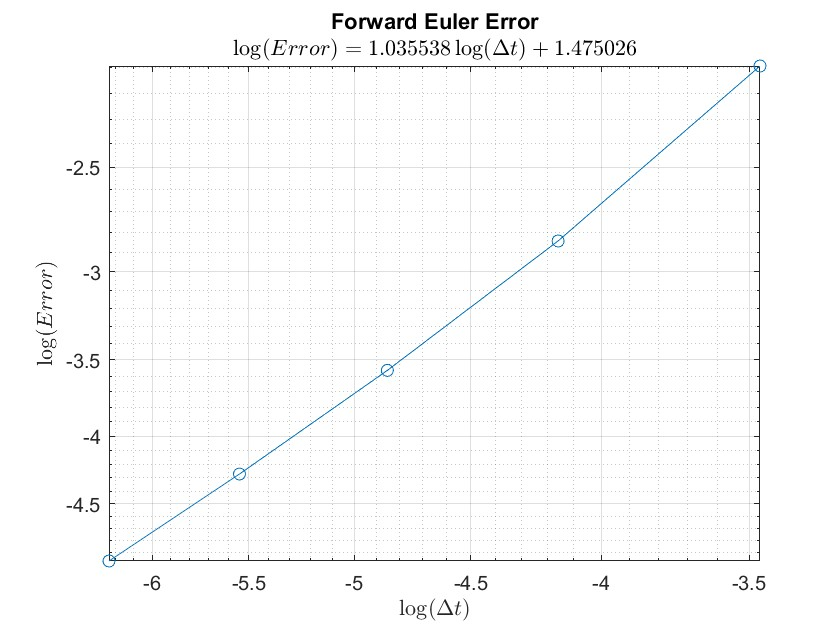
\includegraphics[width = 1\linewidth]{forward_error.jpg}
\end{figure}

The slope of the log-log plot regression properly shows the order of accuracy for the Forward Euler method, which is one. 
This is due to this Forward Euler Method having a schematic error of $\mathcal{O}(\Delta t)$ and a truncation error of $\mathcal{O}(\Delta t^{2})$ 
\newpage
	\item \textbf{Backward Euler}:\\
	
The Backwards Euler Method is defined as\ldots
\begin{equation}
    F(u^{i}) = \frac{u^{i+1}-u^{i}}{\Delta t} \longrightarrow u^{i+1} = u^{i} + \Delta t  F(u^{i+1})
\end{equation}
Rewritten as a system of matrices to be itterated over each time-step, $\Delta t$\ldots
\begin{center} 
    $\begin{bmatrix} 1&0 \\ 0&1 \end{bmatrix} \begin{bmatrix} u_{1} \\ u_{2} \end{bmatrix}^{i+1} = \begin{bmatrix} u_{1} \\ u_{2} \end{bmatrix}^{i} + \begin{bmatrix} 0&\Delta t \\ -2\Delta t &0 \end{bmatrix}\begin{bmatrix} u_{1} \\ u_{2} \end{bmatrix}^{i+1} \hspace{0.5 cm} \longrightarrow \hspace{0.5 cm} \begin{bmatrix} -1&\Delta t \\ 2\Delta t &1 \end{bmatrix} \begin{bmatrix} u_{1} \\ u_{2} \end{bmatrix}^{i+1} = \begin{bmatrix} u_{1} \\ u_{2} \end{bmatrix}^{i}$
\end{center}
\begin{center} 
    $\longrightarrow \hspace{0.5 cm}\begin{bmatrix} u_{1} \\ u_{2} \end{bmatrix}^{i+1} = \begin{bmatrix} -1&\Delta t \\ 2\Delta t &1 \end{bmatrix}^{-1} \begin{bmatrix} u_{1} \\ u_{2} \end{bmatrix}^{i}$
\end{center}

This process is displayed in the function, backward\_euler:
\lstset{title={backward\_euler}}
\begin{lstlisting}[language = Matlab]
function [U, Error] = backward_euler(dt, time)
    steps = time/dt;
    t_vec = [0 : dt : time]; 
    U = zeros(2,steps+1);
    Analytic = U;
    
    % Set initial condition
    U(:, 1) = [1 ; 0];
    
    % finite difference Matrix
    F = [1      -dt;...
         2*dt   1];
    
    % looop over all time steps
    for ii=2:steps
        U(:, ii) = inv(F)*U(:,ii-1);
    end
    
    Analytic (1,:) = analytic(t_vec);
    Analytic (2,:) = analyticdt(t_vec);

    Error = abs( U(1,(end+1)/2) - Analytic(1,(end+1)/2) ); 
end
\end{lstlisting}

Graphs comparing $\frac{du}{dt}$ vs $u$ using the different finite difference methods are located towards the end of the paper.

The Backwards Euler Method tends to swirl inside the analytical result as the error in each progression through time draws itself closer to zero. The error kind of subtracts itself further from the correct answer.


\newpage
A log-log plot of the error compared with the different time-steps, $\Delta t$, is\ldots

\begin{figure}[!h]
    \centering
    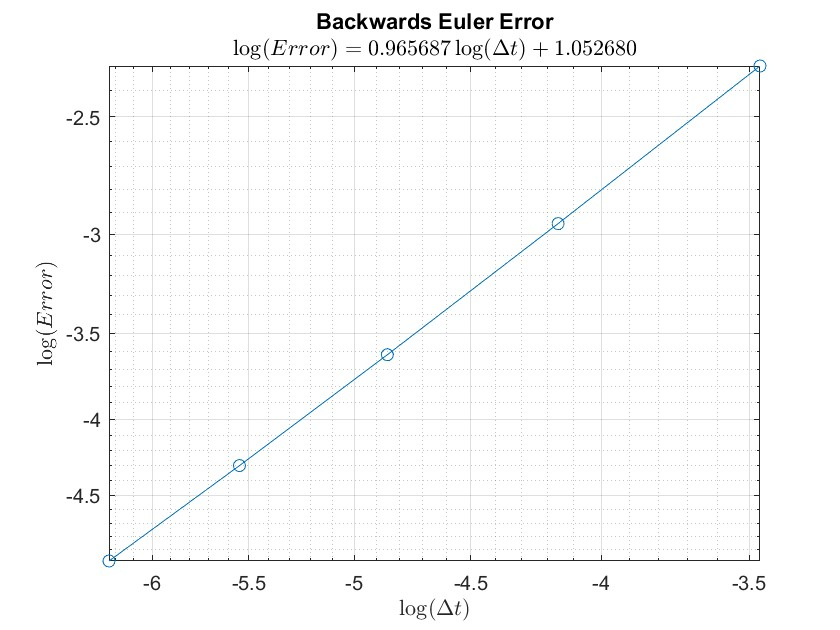
\includegraphics[width = 1\linewidth]{backward_error.jpg}
\end{figure}

The slope of the log-log plot regression properly shows the order of accuracy for the Backwards Euler method, which is one. 
This is due to this Backwards Euler Method having a schematic error of $\mathcal{O}(\Delta t)$ and a truncation error of $\mathcal{O}(\Delta t^{2})$ 
\newpage
	\item \textbf{The Trapezoidal method}:\
	
The Trapezoidal Method is defined as\ldots
\begin{equation}
    u^{i+1} = u^{i} + \frac{\Delta t}{2} \left( F(u^{i}) + F(u^{i+1}) \right)
\end{equation}
Rewritten as a system of matrices to be itterated over each time-step, $\Delta t$\ldots
\begin{center} 
    $\begin{bmatrix} 1&0 \\ 0&1 \end{bmatrix} \begin{bmatrix} u_{1} \\ u_{2} \end{bmatrix}^{i+1} = \begin{bmatrix} 1&0 \\ 0&1 \end{bmatrix} \begin{bmatrix} u_{1} \\ u_{2} \end{bmatrix}^{i} +  \begin{bmatrix} 0&\frac{\Delta t}{2} \\ -\Delta t &0 \end{bmatrix}\begin{bmatrix} u_{1} \\ u_{2} \end{bmatrix}^{i} + \begin{bmatrix} 0&\frac{\Delta t}{2} \\ -\Delta t &0 \end{bmatrix}\begin{bmatrix} u_{1} \\ u_{2} \end{bmatrix}^{i+1}$
\end{center}

\begin{center} 
    $\longrightarrow \hspace{0.5 cm} \begin{bmatrix} 1&\frac{-\Delta t}{2} \\ \Delta t &1 \end{bmatrix} \begin{bmatrix} u_{1} \\ u_{2} \end{bmatrix}^{i+1} = \begin{bmatrix} 1&\frac{\Delta t}{2} \\ -\Delta t &1 \end{bmatrix}\begin{bmatrix} u_{1} \\ u_{2} \end{bmatrix}^{i}$
\end{center}

\begin{center} 
    $\longrightarrow \hspace{0.5 cm}  \begin{bmatrix} u_{1} \\ u_{2} \end{bmatrix}^{i+1} = \begin{bmatrix} 1&\frac{-\Delta t}{2} \\ \Delta t &1 \end{bmatrix}^{-1} \begin{bmatrix} 1&\frac{\Delta t}{2} \\ -\Delta t &1 \end{bmatrix}\begin{bmatrix} u_{1} \\ u_{2} \end{bmatrix}^{i}$
\end{center}

This process is displayed in the function, trapezoid:
\lstset{title={backward\_euler}}
\begin{lstlisting}[language = Matlab]
function [U, Error] = trapezoid(dt, time)
    steps = time/dt;
    t_vec = [0 : dt : time]; 
    U = zeros(2,steps+1);
    Analytic = U;
    
    % Set initial condition
    U(:, 1) = [1 ; 0];
    
    % finite difference Matrices
    F1 = [1      dt/2;...
         -dt     1];
    F2 = [1      -dt/2;...
         dt     1];
    
    % looop over all time steps
    for ii=2:steps
        U(:, ii) = inv(F2)*F1*U(:,ii-1);
    end
    
    Analytic (1,:) = analytic(t_vec);
    Analytic (2,:) = analyticdt(t_vec);

    Error = abs( U(1,(end+1)/2) - Analytic(1,(end+1)/2) ); 
end
\end{lstlisting}

Graphs comparing $\frac{du}{dt}$ vs $u$ using the different finite difference methods are located towards the end of the paper.

The Trapezoidal Method tends to track well with the analytical answer. Being an average of the Forward and Backwards Euler Methods, the error of the Forward Euler Method kind of cancels out the error of the Backwards Euler method. However, that is not to mean that there isn't any error, which is discussed below.

\newpage
A log-log plot of the error compared with the different time-steps, $\Delta t$, is\ldots

\begin{figure}[!h]
    \centering
    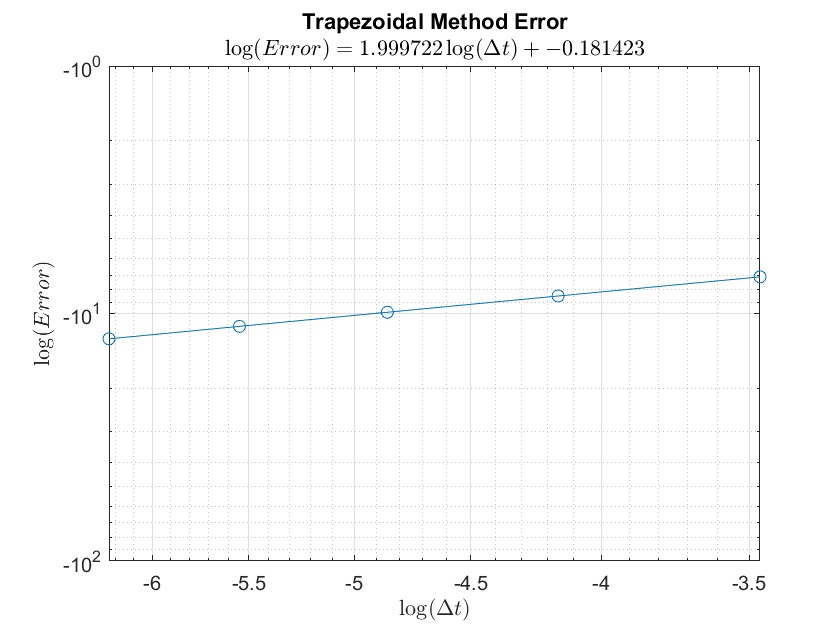
\includegraphics[width = 1\linewidth]{trapezoid_error.jpg}
\end{figure}

The slope of the log-log plot regression properly shows the order of accuracy for the Trapezoidal Method, which is two. 
This is due to this Trapezoidal Method having a schematic error of $\mathcal{O}(\Delta t^{2})$ 

\end{enumerate}


\newpage

\section*{$\frac{du}{dt}$ vs $u$ Comparison Plots}
\begin{figure}[!h]
    \centering
    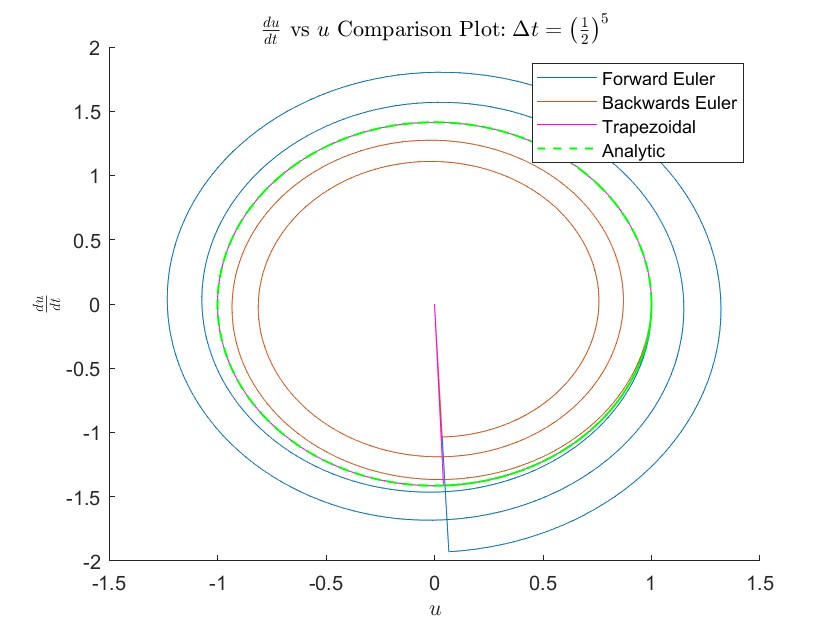
\includegraphics[width = 0.85\linewidth]{dudt_vs_u1.jpg}
    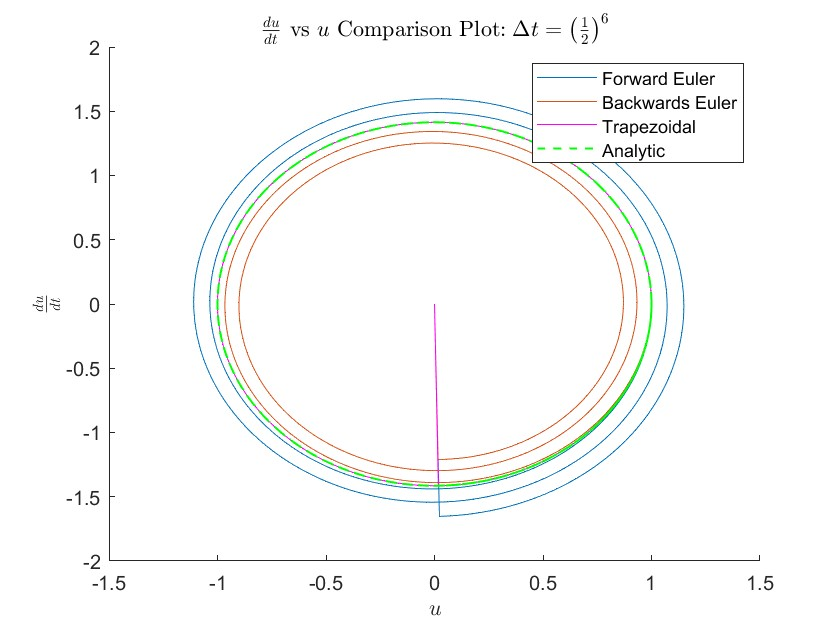
\includegraphics[width = 0.85\linewidth]{dudt_vs_u2.jpg}
\end{figure}
\newpage
\begin{figure}[!h]
    \centering
    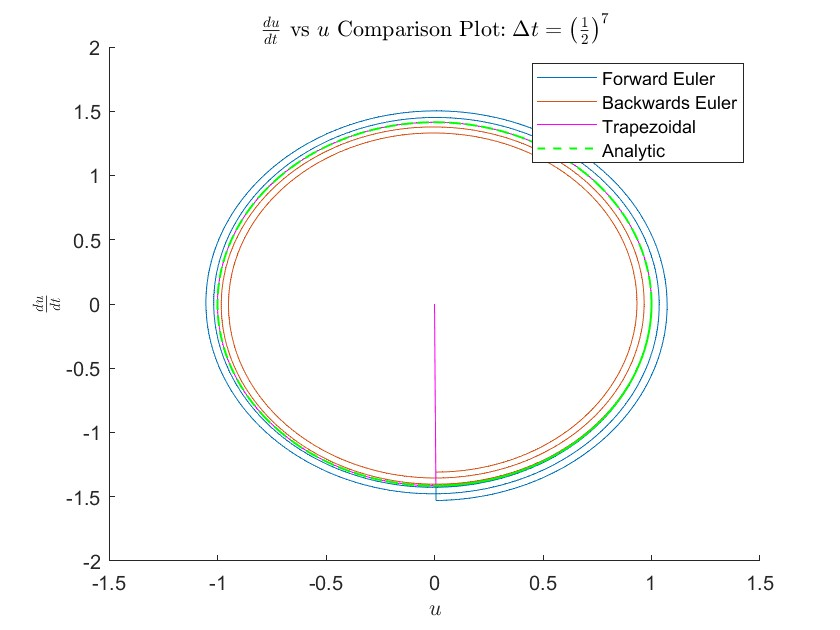
\includegraphics[width = 1\linewidth]{dudt_vs_u3.jpg}
    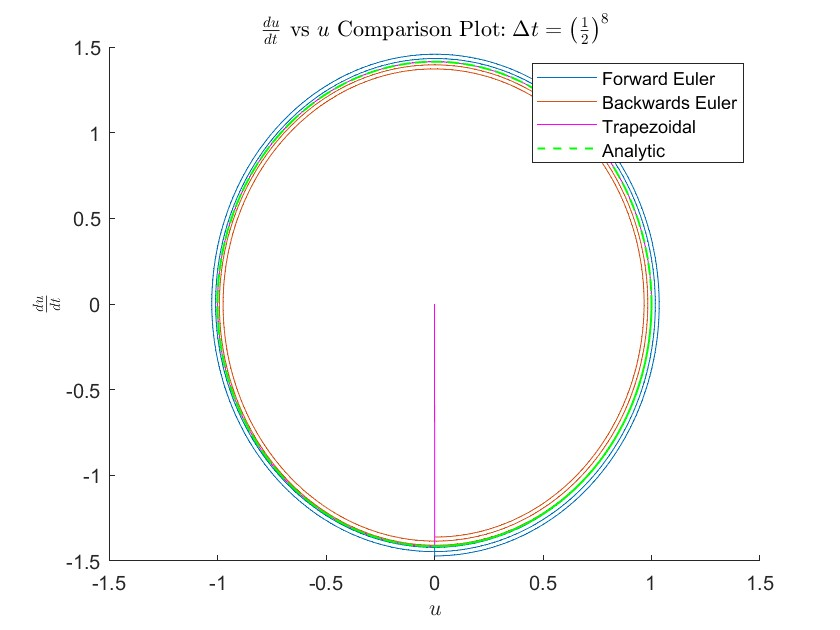
\includegraphics[width = 1\linewidth]{dudt_vs_u4.jpg}
\end{figure}
\newpage
\begin{figure}[!h]
    \centering
    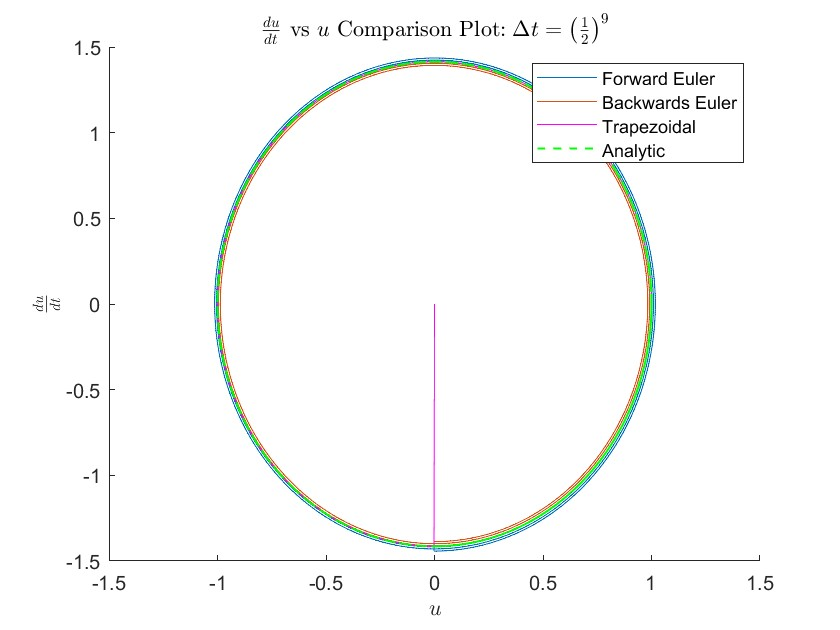
\includegraphics[width = 1\linewidth]{dudt_vs_u5.jpg}
\end{figure}


\clearpage
\section*{Matlab Code}
\begin{lstlisting}[language = Matlab]
%% Zack Humphries
% COMP 521
% HW6

close all;
clear;
clc;

% Analytical solution == u(t) = cos(sqrt(2) * t)
% u(0) = 1
% u'(t) = 0

time = 10;
expo = [5 6 7 8 9];
time_steps = 1./2.^expo;

%%
forward_euler_error = zeros(length(time_steps),1);
backward_euler_error = zeros(length(time_steps),1);
trapezoid_error = zeros(length(time_steps),1);

for kk = 1:length(time_steps)
    
    dt = time_steps(kk);
    t_vec = [0 : dt : time]; 
    [forward_euler_U, Analytic, Error_forward] = forward_euler(dt, time);
    forward_euler_error(kk,1) = Error_forward;

    [backward_euler_U, Error_backward] = backward_euler(dt, time);
    backward_euler_error(kk,1) = Error_backward;

    [trapezoid_U, Error_trapezoid] = trapezoid(dt, time);
    trapezoid_error(kk,1) = Error_trapezoid;

    figure
    hold on
    plot(forward_euler_U(1,:), forward_euler_U(2,:));
    plot(backward_euler_U(1,:), backward_euler_U(2,:));
    plot(trapezoid_U(1,:), trapezoid_U(2,:), '-m');
    plot(Analytic(1,:), Analytic(2,:), '--g', "LineWidth",1);
    title_name = strcat("$\frac{du}{dt}$ vs $u$ Comparison Plot$: \Delta t = \left(\frac{1}{2}\right)^{", sprintf("%i", expo(kk)), "}$");
    title(title_name,'interpreter','latex')
    legend("Forward Euler", "Backwards Euler", "Trapezoidal", "Analytic")
    xlabel("$u$",'interpreter','latex')
    ylabel("$\frac{du}{dt}$",'interpreter','latex')
    % add a legend, label, etc, etc
    hold off
end

%% make plot

% Error plotting
figure
forward_poly = polyfit(log(time_steps), log(forward_euler_error), 1);
loglog(log(time_steps), log(forward_euler_error), "o-"); grid on;
title("Forward Euler Error")
subtitle_name_forward = strcat("$\log(Error) = ", sprintf("%2.6f", forward_poly(1)), "\log(\Delta t) + ", sprintf("%2.6f", forward_poly(2)), "$");
subtitle(subtitle_name_forward,'interpreter','latex')
xlabel("$\log(\Delta t)$",'interpreter','latex')
ylabel("$\log(Error)$",'interpreter','latex')
figure
backward_poly = polyfit(log(time_steps), log(backward_euler_error), 1);
loglog(log(time_steps), log(backward_euler_error), "o-"); grid on;
title("Backwards Euler Error")
subtitle_name_backward = strcat("$\log(Error) = ", sprintf("%2.6f", backward_poly(1)), "\log(\Delta t) + ", sprintf("%2.6f", backward_poly(2)), "$");
subtitle(subtitle_name_backward,'interpreter','latex')
xlabel("$\log(\Delta t)$",'interpreter','latex')
ylabel("$\log(Error)$",'interpreter','latex')
figure
trapezoid_poly = polyfit(log(time_steps), log(trapezoid_error), 1);
loglog(log(time_steps), log(trapezoid_error), "o-"); grid on;
title("Trapezoidal Method Error")
subtitle_name_trapezoid = strcat("$\log(Error) = ", sprintf("%2.6f", trapezoid_poly(1)), "\log(\Delta t) + ", sprintf("%2.6f", trapezoid_poly(2)), "$");
subtitle(subtitle_name_trapezoid,'interpreter','latex')
xlabel("$\log(\Delta t)$",'interpreter','latex')
ylabel("$\log(Error)$",'interpreter','latex')

% HW asks for global trunc error and last time step

%% Forward Euler Function

function [U, Analytic, Error] = forward_euler(dt, time)
    steps = time/dt;
    t_vec = [0 : dt : time]; 
    U = zeros(2,steps+1);
    Analytic = zeros(2,steps+1);
    
    % Set initial condition
    U(:, 1) = [1 ; 0];
    
    % finite difference Matrix
    F = [1      dt;...
        -2*dt   1];
    
    % looop over all time steps
    for ii=2:steps
        U(:, ii) = F * U(:,ii-1);
    end
    
    Analytic (1,:) = analytic(t_vec);
    Analytic (2,:) = analyticdt(t_vec);

    Error = abs( U(1,(end+1)/2) - Analytic(1,(end+1)/2) );
end

%% Backwards Euler Function

function [U, Error] = backward_euler(dt, time)
    steps = time/dt;
    t_vec = [0 : dt : time]; 
    U = zeros(2,steps+1);
    Analytic = U;
    
    % Set initial condition
    U(:, 1) = [1 ; 0];
    
    % finite difference Matrix
    F = [1      -dt;...
         2*dt   1];
    
    % looop over all time steps
    for ii=2:steps
        U(:, ii) = inv(F)*U(:,ii-1);
    end
    
    Analytic (1,:) = analytic(t_vec);
    Analytic (2,:) = analyticdt(t_vec);

    Error = abs( U(1,(end+1)/2) - Analytic(1,(end+1)/2) ); 
end

%% Trapezoid Function

function [U, Error] = trapezoid(dt, time)
    steps = time/dt;
    t_vec = [0 : dt : time]; 
    U = zeros(2,steps+1);
    Analytic = U;
    
    % Set initial condition
    U(:, 1) = [1 ; 0];
    
    % finite difference Matrices
    F1 = [1      dt/2;...
         -dt     1];
    F2 = [1      -dt/2;...
         dt     1];
    
    % looop over all time steps
    for ii=2:steps
        U(:, ii) = inv(F2)*F1*U(:,ii-1);
    end
    
    Analytic (1,:) = analytic(t_vec);
    Analytic (2,:) = analyticdt(t_vec);

    Error = abs( U(1,(end+1)/2) - Analytic(1,(end+1)/2) ); 
end

function result = analytic(t)
    s2 = sqrt(2);
    result = cos(s2 .* t);
end

function result = analyticdt(t)
    s2 = sqrt(2);
    result = -s2 .* sin(s2 .* t);
end
\end{lstlisting}



\end{document}